\documentclass[11pt,a4paper]{article}
\usepackage[utf8]{inputenc}
\usepackage[english]{babel}
\usepackage{amsmath}
\usepackage{amsfonts}
\usepackage{amssymb}
\usepackage{graphicx}
\graphicspath{{../figures/}}
\author{Jacob Heden Malm}
\title{DD2424 Assignment 1}
\begin{document}
\maketitle

\section{Implementation details and success of gradient descent}

I was able to write all of the required functions without issue. In order to verify that my gradient computations were correct, I first debugged the program during its execution and visually compared the gradient values computed by my gradient descent method as well as the numerical approximation method we were given. I then wrote a method called "verify\_gradient\_descent()" that a mini batch of training examples, the weight and bias matrix, a regularization parameter, and a permitted difference. This method then computes the gradient update using the analytic method and the numerical method, and takes the absolute value of the difference matrix computed by the two methods. It then asserts that the means of these two matrices (W and b) are less than the permitted difference parameter. Using a mini batch of 5 data points, and a regularization multiplier of 0.01 I got the mean of the absolute difference to be in the neighborhood of 4.5e-8. I took this to signify success.\\

I chose to randomize the order of training examples between each epoch. I also used all of the available data for training my network, and split the test set into a validation set consisting of 1000 examples, and the rest being the final test set.

\subsection{Data and figures}
Here, graphs detailing the training development and images representing the learnt weight matrix will be shown for the different required parameter settings.

\subsubsection{$lambda=0$, $eta=0.1$}
Final test accuracy: 0.3027

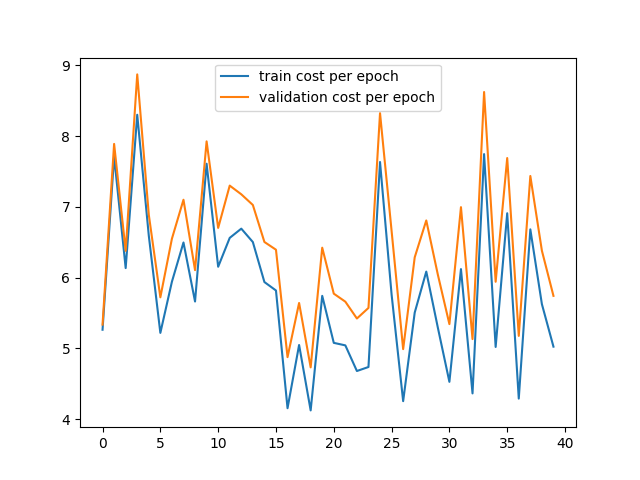
\includegraphics[width=\textwidth]{eta_0.1_lambda_0.png}
As we can see the learning rate here is much too high. This leads to the network never really learning any useful parameters, each new training example changes the parameter settings too much for the network to retain any "knowledge" it has gained from previously seen training examples.

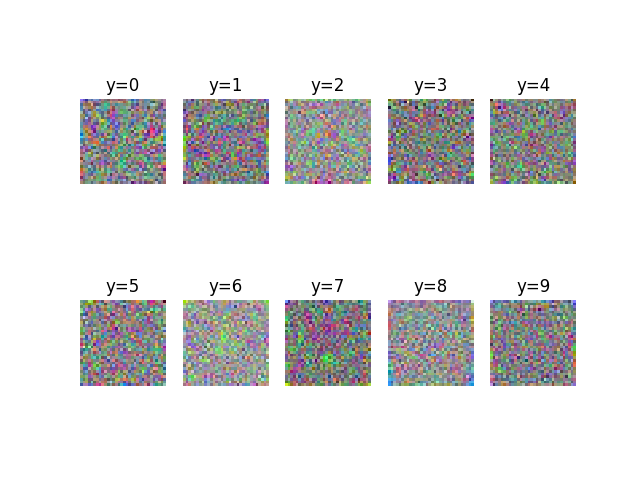
\includegraphics[width=\textwidth]{eta_0.1_lambda_0_montage.png}

These images do not tell us much, they seem to be relatively random blobs of color.


\subsubsection{$lambda=0$, $eta=0.001$}
Final test accuracy: 0.4097

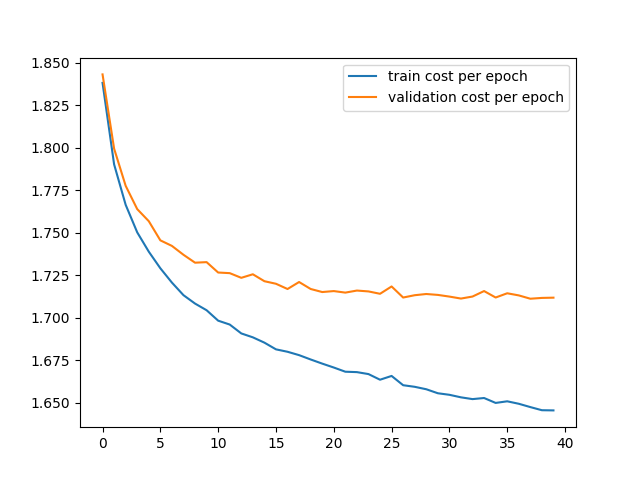
\includegraphics[width=\textwidth]{eta_0.001_lambda_0.png}

Here we can see that this learning rate seems to be a better fit for this network and training data. Especially the training loss seems to decrease steadily as training continues, suggesting that the network continues to get more and more fitted to the training examples we give it.

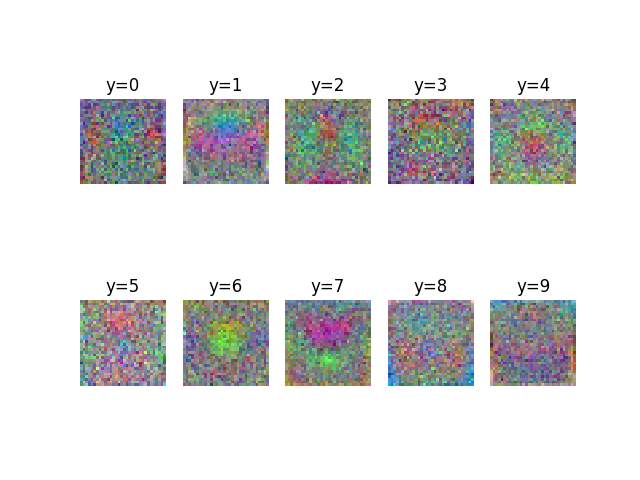
\includegraphics[width=\textwidth]{eta_0.001_lambda_0_montage.png}

We can see clear shapes begin to take form in the learned weight matrix.

\subsubsection{$lambda=0.1$, $eta=0.001$}
Final test accuracy: 0.4095

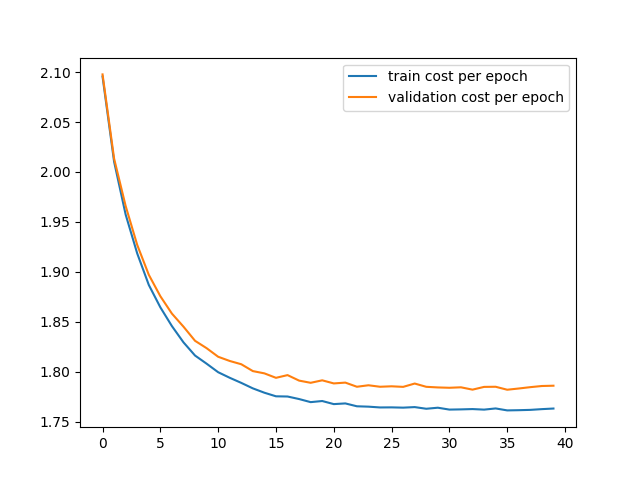
\includegraphics[width=\textwidth]{lambda_0.1.png}

Here we can see the effect of added regularization. Regularization decreases the networks variance, which combats its tendency to overfit. This is demonstrated in the much smaller discrepancy between the networks training and validation loss than in the previous example.

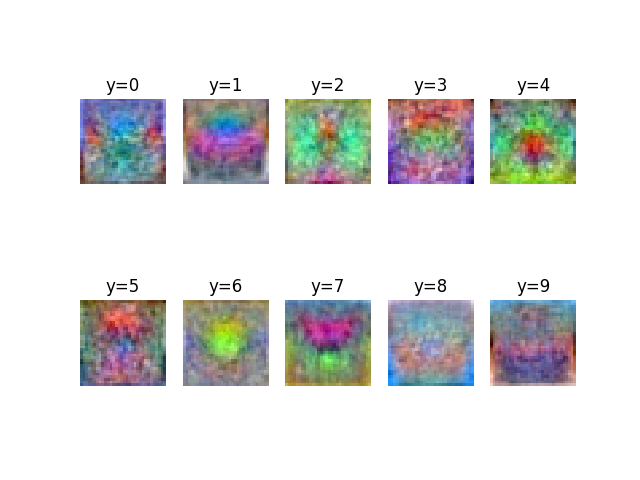
\includegraphics[width=\textwidth]{lambda_0.1_montage.png}

Compared with the previous example, these images look much clearer. The validation accuracies are however more or less equivalent, personally I am not sure how regularization achieves this. Perhaps since increasing the amount of regularization encourages a smoother output function, this results in clearer regions of uniformity in the generated images, essentially encouraging spatial correlation in the pixel values.

\subsubsection{$lambda=1$, $eta=0.001$}
Final test accuracy: 0.3801

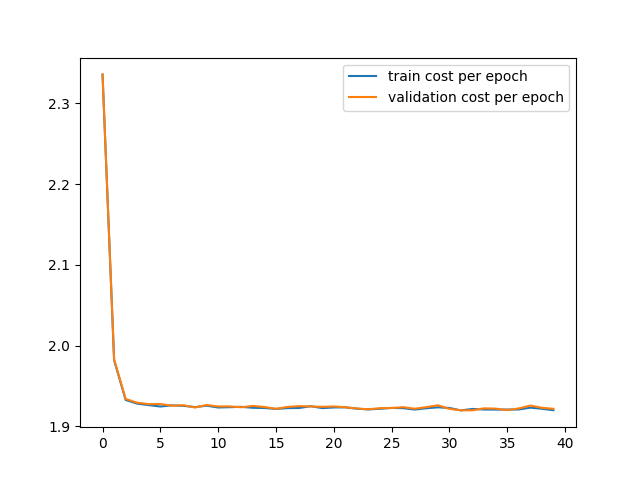
\includegraphics[width=\textwidth]{lambda_1.png}

The aforementioned effects are much more pronounced here. It is however also notable that the loss never reaches as low as it did in the previous example, suggesting that this amount of regularization has introduced too much bias.

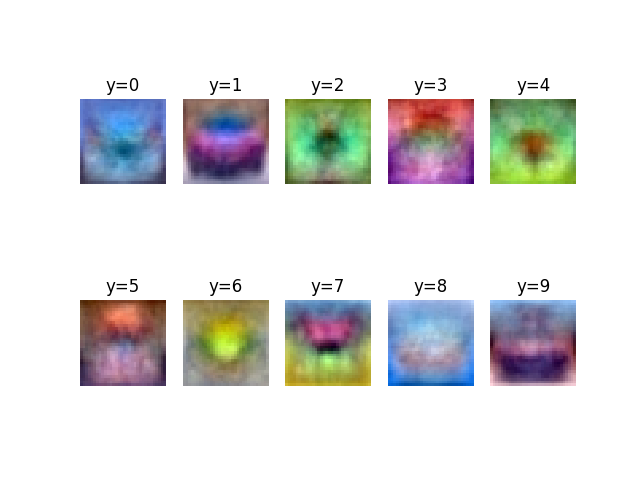
\includegraphics[width=\textwidth]{lambda_1_montage.png}

These images actually look quite good! The lack of noise makes them quite visually appealing in comparison to the previous images. However, noticeably, the test accuracy of this parameter setting is lower than the previous example.

\section{Bonus Points}

\subsection{a, more data}
I was using all 5 batches of training data for all of the above runs, with the validation set consisting of the first 1000 entries in the test set, and the rest being the test set.

However, in order to assess the improvement this change made, I will compare the final test accuracy for a network trained on all batches with the test accuracy of a network trained on only one batch.

\subsubsection{$lambda=0$, $eta=0.1$}
Final test accuracy all batches: 0.3027\\
Final test accuracy batch 1: 0.3064

\subsubsection{$lambda=0$, $eta=0.001$}
Final test accuracy: 0.4097\\
Final test accuracy batch 1: 0.392


\subsubsection{$lambda=0.1$, $eta=0.001$}
Final test accuracy: 0.4095\\
Final test accuracy batch 1: 0.396


\subsubsection{$lambda=1$, $eta=0.001$}
Final test accuracy: 0.3801\\
Final test accuracy batch 1: 0.3734

From these results we can conclude that our network consistently performs slightly better with the expanded data set, given that the learning rate we use to train the network is correct. I did however expect the difference to be much larger than what I observed.

\subsection{b, data augmentation}
I implemented a method to select half the indices of the training set randomly, and a method to horizontally flip these images. The first method, called "flip\_half\_images()" uses the "sample()" method from the python "random" library. It uniformly picks out half the indices within the range of the size of the data set. For each index, we then pass the image to a method called "flip\_image()" which makes use of reshape and transpose numpy methods to reformat the image in the way numpy expects it, and then "numpy.fliplr()" which does the horizontal flip. Additionally, the argument "show\_image=True" can be passed in to visualize the transformation and verify its success.

\subsubsection{$lambda=0$, $eta=0.001$}
Final test accuracy: 0.4153\\
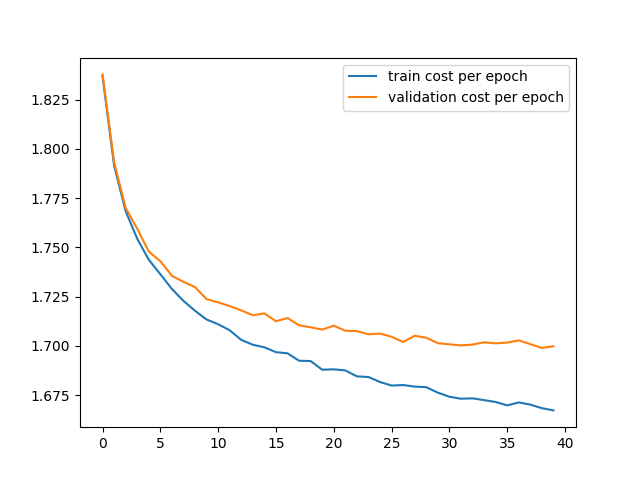
\includegraphics[width=\textwidth]{eta_0.001_lambda_0_augmentation.png}

As we can see the test accuracy here is slightly better than the test accuracy of the corresponding parameter settings without the data augmentation. Interestingly, we can also see that when we compare the two graphs, the validation error both reaches a lower final value, and stays closer to the training performance, indicating that our network does not overfit as much with the data augmentation.


\subsubsection{$lambda=0.1$, $eta=0.001$}
Final test accuracy: 0.4129\\
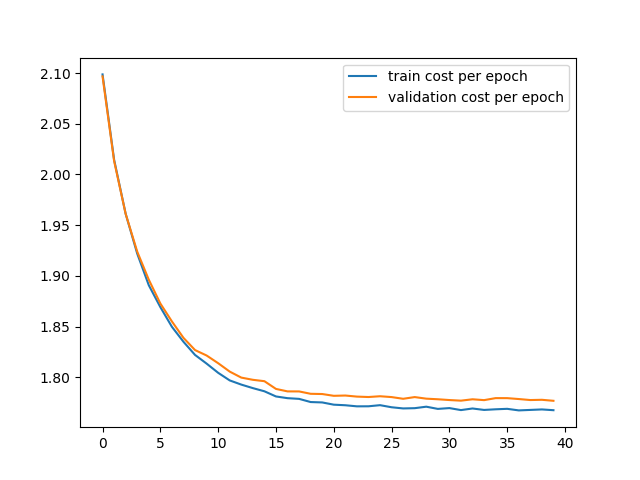
\includegraphics[width=\textwidth]{eta_0.001_lambda_0.1_augmentation.png}

Again, we see proof of the same patterns. A slightly improved test accuracy, as well as a consistently lower validation loss. Overall, the improvement seems to be modest but consistent.

\subsection{c, Grid search for optimal parameter settings}
To solve this problem, I created a method called grid\_search(). This method accepts the same parameters as MiniBatchGD(), with the exception that it also accepts a validation set and that it expects the n\_batches, eta, and lambda parameter to be in the form of lists. We then loop over all combinations of these parameters, and perform a MiniBatchGD(). Then, we take the trained W and b, and assess the validation loss. If the loss is lower than the previously best observed final loss, we update the current saved parameters, and current best observed loss.\\

At the end of trying all these combinations, we return the best parameter combination we observed.\\

I started out by running through these parameters: n\_batches = [50, 100, 200], eta = [0.001, 0.01, 0.1], and lambda = [0, 0.01, 0.1].\\

The combination that was found to produce the lowest validation loss was n\_batch = 200, eta = 0.01, and lambda = 0.\\

This combination resulted in a final test accuracy of 0.4114, which is a little bit lower than previously observed best results, although the difference could very well be due to random fluctuations. Interestingly, this confirms the empirical finding that a slightly higher learning rate can be used with larger batch sizes.\\

In order to find the absolute best combinations, I chose to run another grid search, this time in the neighbourhood of the best combination. Thus I set n\_batches = [150, 200, 250], etas = [0.005, 0.01, 0.015], lambda = [0, 0.0001, 0.005].\\

\end{document}